\documentclass[tikz,border=4pt]{standalone}
\begin{document}
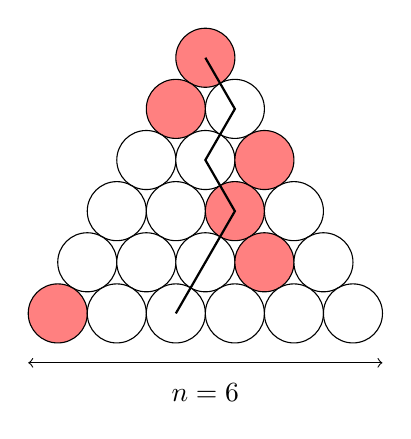
\begin{tikzpicture}[x=.025cm,y=-.025cm]
\draw[fill=red!50] (100,20) circle[radius=.375cm];
\draw[fill=red!50] (85,45.98076211353316) circle[radius=.375cm];
\draw[fill=white] (115,45.98076211353316) circle[radius=.375cm];
\draw[fill=white] (70,71.96152422706632) circle[radius=.375cm];
\draw[fill=white] (100,71.96152422706632) circle[radius=.375cm];
\draw[fill=red!50] (130,71.96152422706632) circle[radius=.375cm];
\draw[fill=white] (55,97.94228634059947) circle[radius=.375cm];
\draw[fill=white] (85,97.94228634059947) circle[radius=.375cm];
\draw[fill=red!50] (115,97.94228634059947) circle[radius=.375cm];
\draw[fill=white] (145,97.94228634059947) circle[radius=.375cm];
\draw[fill=white] (40,123.92304845413263) circle[radius=.375cm];
\draw[fill=white] (70,123.92304845413263) circle[radius=.375cm];
\draw[fill=white] (100,123.92304845413263) circle[radius=.375cm];
\draw[fill=red!50] (130,123.92304845413263) circle[radius=.375cm];
\draw[fill=white] (160,123.92304845413263) circle[radius=.375cm];
\draw[fill=red!50] (25,149.90381056766577) circle[radius=.375cm];
\draw[fill=white] (55,149.90381056766577) circle[radius=.375cm];
\draw[fill=white] (85,149.90381056766577) circle[radius=.375cm];
\draw[fill=white] (115,149.90381056766577) circle[radius=.375cm];
\draw[fill=white] (145,149.90381056766577) circle[radius=.375cm];
\draw[fill=white] (175,149.90381056766577) circle[radius=.375cm];
\draw[thick] (100,20)--(115,45.98076211353316)--(100,71.96152422706632)--(115,97.94228634059947)--(100,123.92304845413263)--(85,149.90381056766577);
\draw[<->] (10,175)--(190,175);
\node at (100,190) {$n=6$};
\end{tikzpicture}
\end{document}
